\documentclass{exam} % {{{1
\usepackage{amsmath, amssymb, amsthm, enumitem, float, caption, mathtools, tikz}
\usetikzlibrary{quantikz, arrows, calc, decorations.markings, matrix, positioning}
\tikzset{>=latex}
\usepackage{stackengine}
\usepackage[final]{hyperref}

% mathbb and mathcal symbols
\newcommand{\NN}{\mathbb{N}}
\newcommand{\ZZ}{\mathbb{Z}}
\newcommand{\QQ}{\mathbb{Q}}
\newcommand{\RR}{\mathbb{R}}
\newcommand{\V}{\mathcal{V}}
\newcommand{\A}{\mathbb{A}}
\newcommand{\m}[1]{\mathbb{#1}}    % for models
\newcommand{\cl}[1]{\mathcal{#1}}  % for classes

% theorems and similar environments
\theoremstyle{plain}
  \newtheorem{thm}{Theorem}[section]  \newtheorem*{thm*}{Theorem}
  \newtheorem{claim}[thm]{Claim}      \newtheorem*{claim*}{Claim}
  \newtheorem{conj}[thm]{Conjecture}  \newtheorem*{conj*}{Conjecture}
  \newtheorem{cor}[thm]{Corollary}    \newtheorem*{cor*}{Corollary}
  \newtheorem{lem}[thm]{Lemma}        \newtheorem*{lem*}{Lemma}
  \newtheorem{prop}[thm]{Proposition} \newtheorem*{prop*}{Proposition}
\theoremstyle{definition}
  \newtheorem{defn}[thm]{Definition} \newtheorem*{defn*}{Definition}
  \newtheorem{ex}[thm]{Example}      \newtheorem*{ex*}{Example}
\theoremstyle{remark}
  \newtheorem{rk}[thm]{Remark}  \newtheorem*{rk*}{Remark}
\newcommand{\Case}[1]{\smallskip \textbf{Case #1:}}
\newenvironment{claimproof} {
  \begin{proof}[Proof of claim]
  \renewcommand{\qedsymbol}{\ensuremath{\circ}}
  } {
  \end{proof}
  }

% custom commands
\DeclareMathOperator{\Cg}{Cg}
\DeclareMathOperator{\Clo}{Clo}
\DeclareMathOperator{\Con}{Con}
\DeclareMathOperator{\Rel}{Rel}
\DeclareMathOperator{\Sg}{Sg}
\DeclareMathOperator{\diag}{diag}
\newcommand{\bmat}[1]{ \begin{bmatrix} #1 \end{bmatrix} }
\newcommand{\Bmat}[1]{ \begin{Bmatrix} #1 \end{Bmatrix} }
\newcommand{\pmat}[1]{ \begin{pmatrix} #1 \end{pmatrix} }
\newcommand{\mat}[1]{ \begin{matrix} #1 \end{matrix} }
\newcommand{\vect}[1]{ \left< #1 \right> }
\newcommand{\ds}[1]{ \displaystyle{#1} }
\newcommand{\stack}[2]{\genfrac{}{}{0pt}{}{#1}{#2}}

% misc
\pagestyle{foot} \cfoot{\thepage}  % page numbering
\numberwithin{equation}{section}  % number equations within sections
\renewcommand{\d}{\;d}
\renewcommand{\epsilon}{\varepsilon}
\renewcommand{\phi}{\varphi}
\newcommand{\TODO}[1]{\noindent\textbf{TODO: #1}}

% exam documentclass settings
% restyle parts and subparts
\renewcommand{\thepartno}{\roman{partno}}
\renewcommand{\thesubpart}{\alph{subpart}}
\renewcommand{\subpartlabel}{(\thesubpart)}
\renewcommand{\subsubpartlabel}{(\thesubsubpart)}
% restyle multiple choice options
\renewcommand{\choicelabel}{\thechoice)}
% true or false questions (use \TFQuestion)
\newcommand{\TrueFalse}{\hspace*{0.25em}\textbf{True}\hspace*{1.25em}\textbf{False}\hspace*{1em}}
\newlength{\mylena} \newlength{\mylenb} \settowidth{\mylena}{\TrueFalse}
\newcommand{\TFQuestion}[1]{
  \setlength{\mylenb}{\linewidth} 
  \addtolength{\mylenb}{-121.15pt}
  \parbox[t]{\mylena}{\TrueFalse}\parbox[t]{\mylenb}{#1}
}

% document specific stuff
\usepackage{booktabs}
\renewcommand{\O}{\mathcal{O}}
\renewcommand{\P}{\texttt{P}}
\newcommand{\NP}{\texttt{NP}}
\newcommand{\CC}{\mathbb{C}}
\newcommand{\B}{\mathcal{B}}
\renewcommand{\bra}[1]{ \left< #1 \right| }
\renewcommand{\ket}[1]{ \left| #1 \right> }
\newcommand{\bracket}[2]{ \left< #1 \mid #2 \right> }
\newcommand{\LambdaMat}{
  \pmat{
    1&0&0&0\\
    0&1&0&0\\
    0&0&0&1\\
    0&0&1&0
  }
}
\newcommand\ooplus{\stackMath\mathbin{\stackinset{c}{0ex}{c}{0ex}{\oplus}{\bigcirc}}}
%----------------------------------------------------------------------------}}}1

\begin{document}
\printanswers
% title header {{{
\title{Quantum Algorithms \\ Homework 8 Solutions}
\author{Patrick Canny}
\date{Due: 2019-04-02}
\maketitle
\thispagestyle{foot}
%----------------------------------------------------------------------------}}}
\section{Book Problems}
\begin{questions}
  \question Exercise 9.1\\
  \begin{solution}
    \begin{proof}
      The proof that the choice of $\epsilon$ does not matter is similar to an
      argument made earlier in the class about the class $BPP$.\\

      It may be useful to note that I will define an operator called $M$ whose
      job is to compute the result of $MAJ_{\oplus}$ with ancillas.\\

      First, take $k$ many applications of the circuit $U$ as described in the
      textbook ($U = U_L\hdots U_2U_1$) because the problem requires that the
      input to $MAJ_{\oplus}$ be the output qubits of $k$ many copies of $U$.\\

      Now, we need to apply $M$ a number of times to the resulting output 
      of $U$. This number of inputs does not necessarily have to equal $k$, so
      let's call it $m$. The reason for doing this is in order to determine if
      an answer apprears as the result of $k$-many applications of $U$.\\

      It is important to note that $U$ computes a function $F$ with a given 
      probability, specifically:
      \[
        \sum_x |\bra{F(x), z}U\ket{x, 0^{N-m}}|^2 \geq 1-\epsilon
      \]

      So by choosing a sufficiently large value for $k$, the probability of
      at least $k/2$ of the same result produced by $U$ will increase. 
    \end{proof}
  \end{solution}
  \question Exercise 9.3\\
  \begin{solution}
    To answer this question, I will show and explain the result of changing the
    basis oon each of the two input qubits.\\

    First, consider the controlled qubit. From the circuit provided in the
    problem, we can see that the controlled qubit can be represented by
    $H[2]\Lambda(\sigma^x)H[2] = (I\otimes H)\Lambda(\sigma^x)(I\otimes H)$
    which can be used to compute:
    \begin{align*}
      (H\otimes I)\Lambda(\sigma^x)(H\otimes I)
      &=
      1/\sqrt{2}
      \pmat{ 
      1&1&0&0\\
      1&-1&0&0\\
      0&0&1&1\\
      0&0&1&-1
      }
      \LambdaMat
      \pmat{ 
      1&1&0&0\\
      1&-1&0&0\\
      0&0&1&1\\
      0&0&1&-1
      }
      1/\sqrt{2}\\
      &=
      1/2
      \pmat{ 
      1&1&0&0\\
      1&-1&0&0\\
      0&0&1&1\\
      0&0&1&-1
      }
      \pmat{ 
      1&1&0&0\\
      1&-1&0&0\\
      0&0&1&-1\\
      0&0&1&1
      }\\
      &=
      1/2
      \pmat{ 
      2&0&0&0\\
      0&2&0&0\\
      0&0&2&0\\
      0&0&0&-2
      } 
      =
      \pmat{ 
      1&0&0&0\\
      0&1&0&0\\
      0&0&1&0\\
      0&0&0&-1
      } \\
    \end{align*}
    This implies that when the basis is changed for the controlled qubit, it
    is equivilent to leaving the basis unchanged aside from $\ket{1,1}$,
    which is multiplied by $-1$. This matrix is actually the same as $\Lambda
    (\sigma^z)$, which can be seen by extending the pattern of adding $1$s on 
    the diagonal above the Unitary operator $\sigma^z$ as seen with $\Lambda
    (\sigma^x)$.\\

    Now, we can consider the case of $H[1]\Lambda(\sigma^x)H[1] = (H\otimes I)
    \Lambda(\sigma^x)(H\otimes I)$, representing a change of basis on the 
    control qubit:
    \begin{align*}
      (H\otimes I)\Lambda(\sigma^x)(H\otimes I)
      &=
      1/\sqrt{2}
      \pmat{
        1&0&1&0\\
        0&1&0&1\\
        1&0&-1&0\\
        0&1&0&-1
      }
      \LambdaMat
      \pmat{
        1&0&1&0\\
        0&1&0&1\\
        1&0&-1&0\\
        0&1&0&-1
      }
      1/\sqrt{2}\\
      &=
      1/2
      \pmat{
        1&0&1&0\\
        0&1&0&1\\
        1&0&-1&0\\
        0&1&0&-1
      }
      \pmat{
        1&0&1&0\\
        0&1&0&1\\
        0&1&0&-1\\
        1&0&-1&0
      }\\
      &=
      1/2
      \pmat{
        1&1&1&-1\\
        1&1&-1&1\\
        1&-1&1&1\\
        -1&1&1&1
      }\\
    \end{align*}
    This seems to represent multiple rotations about the x axis for a given 
    input qubit.
  \end{solution}
\end{questions}
%----------------------------------------------------------------------------}}}
\section{Additional Problems}
\begin{questions}
% reversible circuits   {{{1
\question Recall the operator $Z$ from page 85 of the text,
\begin{align*}
  Z\ket{a_0,\dots, a_n} 
    &= \ket{a_0\oplus f(a_1,\dots,a_n), a_1,\dots, a_n}, && \text{where} \\
  f(a_1,\dots,a_n)
    &= \begin{cases}
      1 & \text{if } a_1 = \cdots = a_n = 0, \\
      0 & \text{if } \exists j : a_j\neq 0.
    \end{cases}
\end{align*}
Find the matrix for $Z$ when $n = 2$ and prove that it is unitary.
\begin{solution}
  Take the definition of $Z$ when $n = 2$:
  \begin{align*}
    Z\ket{a_0, a_1, a_2} &= \ket{a_0\oplus f(a_1, a_2), (a_1, a_2)}\\
    f(a_1, a_2) 
    &= 
    \begin{cases}
      1 & \text{if } a_1 = a_2 = 0,\\
      0 & \text{if } \exists j:a_j \neq 0.
    \end{cases}
  \end{align*}
  From here, we can build the matrix representation for $Z$ by considering all
  3-qubit basis vectors:
  \begin{align*}
    Z\ket{0,0,0} &= \ket{1,0,0} \quad Z\ket{0,0,1} = \ket{0,0,1}\\
    Z\ket{0,1,0} &= \ket{0,1,0}\quad Z\ket{0,1,1} = \ket{0,1,1}\\
    Z\ket{0,0,0} &= \ket{1,0,0}\quad Z\ket{1,0,1} =\ket{1,0,1} \\
    Z\ket{1,1,0} &=\ket{1,1,0} \quad Z\ket{1,1,1} = \ket{1,1,1}\\
  \end{align*}
  So, the columns of the matrix representation of $Z$ can be given by considering
  these resulting vectors as columns for the matrix. For example, the first 
  column of the matrix will be given by $Z\ket{0,0,0}$ because the basis for the
  new matrix will be lexigraphically ordered in terms of the previous 
  computations. This yields:
  \[
    Z = \pmat{
      0&0&0&0&1&0&0&0\\
      0&1&0&0&0&0&0&0\\
      0&0&1&0&0&0&0&0\\
      0&0&0&1&0&0&0&0\\
      1&0&0&0&0&0&0&0\\
      0&0&0&0&0&1&0&0\\
      0&0&0&0&0&0&1&0\\
      0&0&0&0&0&0&0&1\\
    }
  \]
  To prove that it is a unitary matrix, we must show that it's rows and columns
  are orthonormal.
  \begin{claim} $Z$ is orthonormal
    \begin{claimproof}
      $Z$ is a matrix where every column and every row has exactly a single $1$.
      To show that each column is normal, take it's inner product with itself.\\

      Take $\ket{\chi}$ to be a given column in $Z$.
      \[
        \bracket{\chi}{\chi} = 1
      \]

      To show that all the columns are orthogonal to each other, consider that
      the inner product of a pair of columns. Column $a$ has single $1$ 
      in position $i$ vs column $b$ where that $1$ exists in position $j$, 
      $i\neq j$.\\

      It holds in $Z$ that all pairs of columns hold this property. In computing
      the inner product of two columns that share this property, a $0$ will
      exist in column $b$ at position $i$, and a $0$ will exist in column $a$
      at position $j$. This implies that any $1$ will become a $0$ when 
      computing the inner product of $a$ and $b$. Since all the inner products
      are $0$, it holds that $Z$ is orthogonal.\\

      Since $Z$ is orthonormal, $Z$ is unitary.
    \end{claimproof}
  \end{claim}
\end{solution}
%----------------------------------------------------------------------------}}}1
% reversible circuits   {{{1
\question Define the Boolean function $f: \{0,1\}^2 \to \{0,1\}$ by the
table below (variable $x$ is the horizontal variable and $y$ is vertical).
\[ \begin{array}{c|cc}
  (x,y) & 0 & 1 \\ \midrule
  0     & 1 & 0 \\
  1     & 1 & 1 \\
\end{array} \]
\begin{parts}
  \part Find a boolean circuit that computes $f_{\oplus}$ over the usual
  basis.

  \part Find the matrix for $\widehat{f_{\oplus}}$ relative to the standard
  computational basis.

  \part Find a quantum circuit that computes $\widehat{f_\oplus}$. You may
  use any $2$-qubit gate as well as controlled gates. There is a solution
  without ancillas, but you may use ancillas if you need to.
\end{parts}
\begin{solution}
  \begin{parts}
    \part
    $f_\oplus(x,y,z) = (x,y,z\oplus f(x,y))$, so:
    \begin{align*}
      f_\oplus(0,1,z) &= (0,1,z)\\
      f_\oplus(x,y,z) &= (x,y,\neg z)\\
    \end{align*}
    If we consider the usual basis to be $\{\land, \lor, \neg\}$, the
    reversible basis can be defined as:
    \[
      \{\land_{\oplus}, \lor_{\oplus}, \neg_{\oplus}, \ooplus\}
    \]
    We can now use these gates to construct a reversible boolean circuit:\\
    \begin{center}
      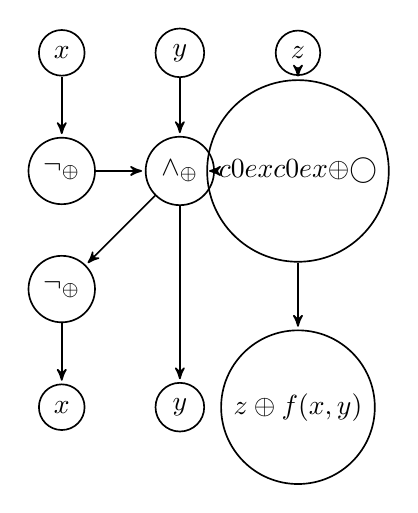
\begin{tikzpicture}[->,
                          >=stealth',
                          ,shorten >=1pt, auto,
                          node distance=1.5cm,
                          semithick, draw=none]
        \tikzstyle{every node} = [circle, draw]
        \node(x) {$x$};
        \node(y)[right of=x] {$y$};
        \node(z)[right of=y] {$z$};
        \node(NOT1)[below of=x] {$\neg_\oplus$};
        \node(AND)[right of=NOT1] {$\land_\oplus$};
        \node(XOR)[right of=AND] {$\ooplus$};
        \node(NOT2)[below of=NOT1] {$\neg_\oplus$};
        \node(x2)[below of=NOT2] {$x$};
        \node(y2)[right of=x2] {$y$};
        \node(OUT)[right of=y2] {$z\oplus f(x,y)$};

        \path (x) edge (NOT1)
              (y) edge (AND)
              (z) edge (XOR)
              (NOT1) edge (AND)
              (AND) edge (NOT2)
                    edge (y2)
                    edge (XOR)
              (NOT2) edge (x2)
              (XOR) edge (OUT);
      \end{tikzpicture}
    \end{center}
    \part
    Similarly to AP 1, $\widehat{f_\oplus}$ can be represented in the 
    3-qubit space by
    considering the solution bits as the result of $f_\oplus$ applied to a 
    3-qubit basis vector representing the input to $f_\oplus$:
    \begin{align*}
    Z\ket{0,0,0} &= \ket{0,0,1} \quad Z\ket{0,0,1} = \ket{0,0,0}\\
    Z\ket{0,1,0} &= \ket{0,1,1}\quad Z\ket{0,1,1} = \ket{0,1,0}\\
    Z\ket{1,0,0} &= \ket{1,0,1}\quad Z\ket{1,0,1} =\ket{1,0,0} \\
    Z\ket{1,1,0} &=\ket{1,1,1} \quad Z\ket{1,1,1} = \ket{1,1,0}\\
    \end{align*}
    Using the same rationale as AP 1, the resulting matrix for 
    $\widehat{f_\oplus}$ can be established as:
    \[
      f_\oplus =
      \pmat{
        0&1&0&0&0&0&0&0\\
        1&0&0&0&0&0&0&0\\
        0&0&1&0&0&0&0&0\\
        0&0&0&1&0&0&0&0\\
        0&0&0&0&0&1&0&0\\
        0&0&0&0&1&0&0&0\\
        0&0&0&0&0&0&0&1\\
        0&0&0&0&0&0&1&0\\
      }
    \]
    \part
    The quantum circuit for $\widehat{f_\oplus}$ can be represented as:\\
    \begin{center}
      \begin{tikzcd}
        \lstick{$\ket{x}$}&
        \qw&\gate{{\sigma^x}^{-1}}&\ctrl{2}&\qw&\gate{ {\sigma^x}}&\qw&
        \rstick{$\ket{x}$}
        \\
        \lstick{$\ket{y}$}&
        \qw&\qw&\ctrl{1}&\qw&\qw&\qw&\rstick{$\ket{y}$}
        \\
        \lstick{$\ket{z\oplus f_\oplus(x,y)}$}&
        \qw&\qw &\gate{\Lambda^2(\sigma^x)}\hphantom{wide}&\qw&\qw&\qw& 
        \rstick{$\ket{z}$}  
      \end{tikzcd}
    \end{center}
    Where both $\ket{x}, \ket{y}$ are inputs to the Toffoli gate.
  \end{parts}
\end{solution}
%----------------------------------------------------------------------------}}}1
% reversible circuits   {{{1
\question Let $g:\{0,1\}^n\to\{0,1\}^n$ be a reversible boolean function.
Prove that $\widehat{g}$ is unitary.
\begin{solution}
  \begin{proof}
    $\widehat{g}$ provides insight into a pattern that is present when 
    considering a concrete implementation of $g_{\oplus}$:
    \begin{align*}
      g(a_0,a_1\hdots,a_n, c) &= (c\oplus g(a_0,a_1,\hdots,a_n), 
      a_0,a_1,\hdots,a_n)\\
      \widehat{g}\ket{a_0,a_1\hdots,a_n, c} &= \ket{c\oplus g(a_0,a_1,
      \hdots,a_n), 
      a_0,a_1,\hdots,a_n}
    \end{align*}
    So, it holds that the application of $\widehat{g}$ must preserve the 
    original input into $g$.\\
    
    If we recall that the application of any
    operator to an input qubit represents a rotation in the quantum space,
    it follows that whatever operator rotates the input must also be able to
    rotate it back its original position. Call the operator that acts on the
    qubit $\ket{\alpha}$ $U$, the result of this application $\ket{\beta}$,
    and the operator that rotates $\ket{\beta}$ back to $\ket{\alpha}$, $G$.
    The following relationship can be established:
    \[
      GU\ket{\alpha} = \ket{\alpha}
    \]
    So it holds that $GU = I$. Recall that unitary operators have the property
    \[
      U^{\dagger}U = UU^{\dagger} = I
    \]
    $U$ also has the property where $U^{-1} = U^\dagger$. $U$ also preserves
    the norm of a vector, so the result of applying $U$ to a vector will 
    represent a pure rotation about the Bloch sphere without any changes to
    the length of the vector. This implies that $GU$ will only allow 
    $\ket{\beta}$ to remain on the Bloch sphere if both $G$ and $U$ are 
    unitary.\\

    Since $U$ has a unique inverse that which must also be unitary (in order to 
    retain a position on the bloch sphere), it 
    holds
    that $G$ must be $U^\dagger = U^{-1}$.
  \end{proof}
\end{solution}
%----------------------------------------------------------------------------}}}1
\end{questions} \end{document}
